% Copyright 2026 Nobin Sijo (NobinSijo7T).
% SPDX-License-Identifier: Apache-2.0
\documentclass[aspectratio=169,10pt]{beamer}
\usetheme{Madrid}
\usepackage[T1]{fontenc}
\usepackage{lmodern}
\usepackage{amsmath,amssymb}
\usepackage{adjustbox}
\usepackage{tikz}
\usetikzlibrary{shapes.geometric,arrows.meta,positioning,calc,fit,backgrounds}

% Lavender Color Palette for Professional Presentation
\definecolor{lavenderDark}{RGB}{76, 51, 122}
\definecolor{lavenderMedium}{RGB}{124, 98, 173}
\definecolor{lavenderLight}{RGB}{243, 239, 252}
\definecolor{lavenderBorder}{RGB}{186, 168, 224}

\setbeamercolor{frametitle}{bg=lavenderDark,fg=white}
\setbeamertemplate{navigation symbols}{}
\setbeamertemplate{footline}{}

\begin{document}

\begin{frame}[t]{End-to-End System Flowchart (Figure 1.3)}
\vspace{-0.35em}
\centering
\adjustbox{max width=0.98\linewidth, max height=0.88\textheight, keepaspectratio}{%
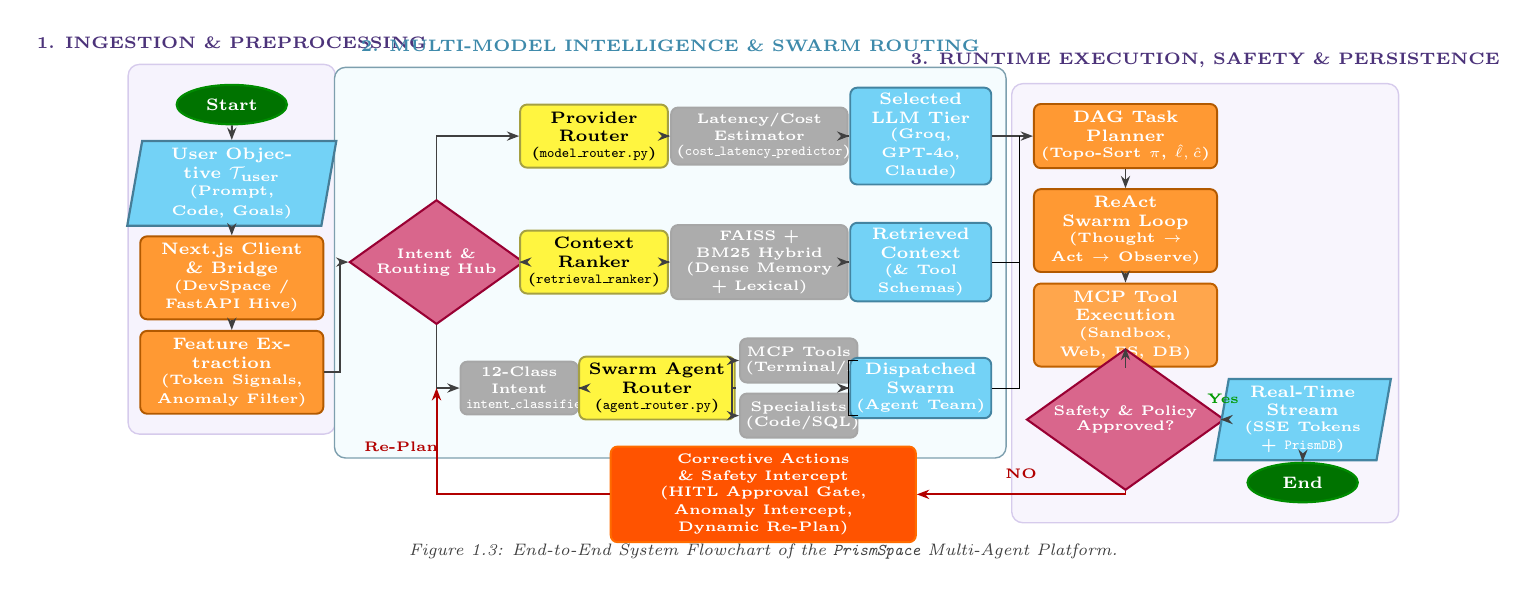
\begin{tikzpicture}[
  x=1cm, y=1cm,
  font=\sffamily,
  % Node styles
  terminal/.style={
    ellipse, draw=green!55!black, fill=green!45!black, text=white,
    line width=0.8pt, inner sep=2.5pt, font=\fontsize{6.5}{7.5}\selectfont\bfseries,
    minimum width=1.4cm, minimum height=0.50cm
  },
  io/.style={
    trapezium, trapezium left angle=80, trapezium right angle=100,
    draw=cyan!55!black, fill=cyan!55, text=white,
    line width=0.8pt, inner sep=2.5pt, font=\fontsize{6.0}{7.0}\selectfont\bfseries,
    minimum width=2.1cm, minimum height=0.52cm, align=center
  },
  proc/.style={
    rectangle, rounded corners=2.5pt,
    draw=orange!70!black, fill=orange!80, text=white,
    line width=0.7pt, inner sep=2.5pt, font=\fontsize{5.8}{6.8}\selectfont\bfseries,
    minimum height=0.60cm, align=center
  },
  branchbox/.style={
    rectangle, rounded corners=2.5pt,
    draw=yellow!60!black, fill=yellow!75, text=black,
    line width=0.7pt, inner sep=2.5pt, font=\fontsize{5.6}{6.6}\selectfont\bfseries,
    minimum height=0.58cm, align=center
  },
  storebox/.style={
    rectangle, rounded corners=2.5pt,
    draw=gray!70, fill=gray!65, text=white,
    line width=0.7pt, inner sep=2pt, font=\fontsize{5.2}{6.2}\selectfont\bfseries,
    minimum height=0.56cm, align=center
  },
  docbox/.style={
    rectangle, rounded corners=2.5pt,
    draw=cyan!60!black, fill=cyan!55, text=white,
    line width=0.7pt, inner sep=2pt, font=\fontsize{5.6}{6.6}\selectfont\bfseries,
    minimum height=0.56cm, align=center
  },
  decision/.style={
    diamond, aspect=1.40,
    draw=purple!80!black, fill=purple!60, text=white,
    line width=0.75pt, inner sep=1.2pt, font=\fontsize{5.2}{6.2}\selectfont\bfseries,
    minimum width=1.55cm, minimum height=0.74cm, align=center
  },
  llmbox/.style={
    rectangle, rounded corners=2.5pt,
    draw=orange!75!black, fill=orange!70, text=white,
    line width=0.7pt, inner sep=2.5pt, font=\fontsize{5.8}{6.8}\selectfont\bfseries,
    minimum height=0.60cm, align=center
  },
  correctbox/.style={
    rectangle, rounded corners=2.5pt,
    draw=orange!85!red, fill=orange!65!red, text=white,
    line width=0.7pt, inner sep=2.5pt, font=\fontsize{5.4}{6.4}\selectfont\bfseries,
    minimum height=0.54cm, align=center
  },
  outbox/.style={
    trapezium, trapezium left angle=80, trapezium right angle=100,
    draw=cyan!60!black, fill=cyan!55, text=white,
    line width=0.8pt, inner sep=2.5pt, font=\fontsize{5.6}{6.6}\selectfont\bfseries,
    minimum width=1.85cm, minimum height=0.52cm, align=center
  },
  stagehdr/.style={
    font=\fontsize{5.8}{6.8}\selectfont\bfseries, text=lavenderDark
  },
  % Arrows
  arr/.style={-{Stealth[scale=0.72]}, line width=0.70pt, draw=black!75},
  redarr/.style={-{Stealth[scale=0.72]}, line width=0.72pt, draw=red!70!black},
]

% =========================================================================
% STAGE 1: INGESTION & PREPROCESSING (Left Column, x = 1.05)
% =========================================================================
\node[terminal] (start) at (1.05, 4.85) {Start};
\node[io, text width=2.10cm]   (uq)    at (1.05, 3.85) {\textbf{User Objective} $\mathcal{T}_{\text{user}}$\\[-0.10em]{\fontsize{4.4}{5.2}\selectfont(Prompt, Code, Goals)}};
\node[proc, text width=2.15cm] (agent) at (1.05, 2.65) {Next.js Client \& Bridge\\[-0.10em]{\fontsize{4.4}{5.2}\selectfont(DevSpace / FastAPI Hive)}};
\node[proc, text width=2.15cm] (qpre)  at (1.05, 1.45) {Feature Extraction\\[-0.10em]{\fontsize{4.4}{5.2}\selectfont(Token Signals, Anomaly Filter)}};

\draw[arr] (start) -- (uq);
\draw[arr] (uq)    -- (agent);
\draw[arr] (agent) -- (qpre);

% =========================================================================
% STAGE 2: MULTI-MODEL INTELLIGENCE & SWARM ROUTING (Center)
% =========================================================================
% Decision Node: Intent & Routing Hub
\node[decision] (sdn) at (3.65, 2.85) {Intent \&\\[-0.10em]Routing Hub};

% Arrow from Preprocessing to Routing Hub
\draw[arr] (qpre.east) -- (2.42, 1.45) -- (2.42, 2.85) -- (sdn.west);

% --- Branch 1: Model Provider Routing (Top row, y = 4.45) ---
\node[branchbox, text width=1.70cm] (kw)    at (5.65, 4.45) {Provider Router\\[-0.10em]{\fontsize{4.3}{5.1}\selectfont(\texttt{model\_router.py})}};
\node[storebox,  text width=2.10cm] (kwst)  at (7.75, 4.45) {Latency/Cost Estimator\\[-0.10em]{\fontsize{4.2}{5.0}\selectfont(\texttt{cost\_latency\_predictor})}};
\node[docbox,    text width=1.65cm] (kwret) at (9.80, 4.45) {Selected LLM Tier\\[-0.10em]{\fontsize{4.2}{5.0}\selectfont(Groq, \mbox{GPT-4o}, Claude)}};

\draw[arr] (sdn.north) -- (3.65, 4.45) -- (kw.west);
\draw[arr] (kw)   -- (kwst);
\draw[arr] (kwst) -- (kwret);

% --- Branch 2: Context & Memory Retrieval (Middle row, y = 2.85) ---
\node[branchbox, text width=1.70cm] (sem)   at (5.65, 2.85) {Context Ranker\\[-0.10em]{\fontsize{4.3}{5.1}\selectfont(\texttt{retrieval\_ranker})}};
\node[storebox,  text width=2.10cm] (semst) at (7.75, 2.85) {FAISS + BM25 Hybrid\\[-0.10em]{\fontsize{4.2}{5.0}\selectfont(Dense Memory + Lexical)}};
\node[docbox,    text width=1.65cm] (semret)at (9.80, 2.85) {Retrieved Context\\[-0.10em]{\fontsize{4.2}{5.0}\selectfont(\& Tool Schemas)}};

\draw[arr] (sdn.east) -- (sem.west);
\draw[arr] (sem)   -- (semst);
\draw[arr] (semst) -- (semret);

% --- Branch 3: Swarm Specialist Dispatch (Bottom row, y = 1.25) ---
\node[storebox,  text width=1.35cm] (embm)  at (4.70, 1.25) {12-Class Intent\\[-0.10em]{\fontsize{4.1}{4.9}\selectfont\texttt{intent\_classifier}}};
\node[branchbox, text width=1.80cm] (hyb)   at (6.45, 1.25) {Swarm Agent Router\\[-0.10em]{\fontsize{4.3}{5.1}\selectfont(\texttt{agent\_router.py})}};
\node[storebox,  text width=1.35cm] (hybkw) at (8.25, 1.60) {MCP Tools\\[-0.10em]{\fontsize{4.0}{4.8}\selectfont(Terminal/FS)}};
\node[storebox,  text width=1.35cm] (hybsem)at (8.25, 0.90) {Specialists\\[-0.10em]{\fontsize{4.0}{4.8}\selectfont(Code/SQL)}};
\node[docbox,    text width=1.65cm] (hybret)at (9.80, 1.25) {Dispatched Swarm\\[-0.10em]{\fontsize{4.2}{5.0}\selectfont(Agent Team)}};

\draw[arr] (sdn.south) -- (3.65, 1.25) -- (embm.west);
\draw[arr] (embm) -- (hyb);
\draw[arr] (hyb.east) -- (7.40, 1.25) |- (hybkw.west);
\draw[arr] (hyb.east) -- (7.40, 1.25) |- (hybsem.west);
\draw[-]   (hybkw.east) -| (8.88, 1.25);
\draw[-]   (hybsem.east)-| (8.88, 1.25);
\draw[arr] (8.88, 1.25) -- (hybret.west);

% =========================================================================
% STAGE 3: EXECUTION, SAFETY & LOCAL PERSISTENCE (Right Column)
% =========================================================================
\node[proc,   text width=2.15cm] (irf)   at (12.4, 4.45) {DAG Task Planner\\[-0.10em]{\fontsize{4.4}{5.2}\selectfont(Topo-Sort $\pi$, $\hat{\ell}, \hat{c}$)}};
\node[proc,   text width=2.15cm] (dedup) at (12.4, 3.25) {ReAct Swarm Loop\\[-0.10em]{\fontsize{4.2}{5.0}\selectfont(Thought $\to$ Act $\to$ Observe)}};
\node[llmbox, text width=2.15cm] (llm)   at (12.4, 2.05) {MCP Tool Execution\\[-0.10em]{\fontsize{4.4}{5.2}\selectfont(Sandbox, Web, FS, DB)}};
\node[decision]                  (verify)at (12.4, 0.85) {Safety \& Policy\\[-0.10em]Approved?};

% Intelligence outputs to DAG Planner bus connection (gap between Stage 2 and 3)
\draw[arr] (kwret.east) -- (11.05, 4.45) -- (irf.west);
\draw[-]   (semret.east) -- (11.05, 2.85) -- (11.05, 4.45);
\draw[-]   (hybret.east) -- (11.05, 1.25) -- (11.05, 2.85);

% Downward flow in Stage 3
\draw[arr] (irf)   -- (dedup);
\draw[arr] (dedup) -- (llm);
\draw[arr] (llm)   -- (verify);

% Verification: YES -> Real-Time Delivery & End
\node[outbox,   text width=1.70cm] (fout) at (14.65, 0.85) {Real-Time Stream\\[-0.10em]{\fontsize{4.3}{5.1}\selectfont(SSE Tokens + \texttt{PrismDB})}};
\node[terminal]                    (endn) at (14.65, 0.05) {End};

\draw[arr] (verify.east) -- node[above=2pt, font=\fontsize{5.2}{6.2}\selectfont\bfseries, text=green!60!black, midway]{Yes} (fout.west);
\draw[arr] (fout) -- (endn);

% Verification: NO -> Corrective Actions & Re-Plan Loop
\node[correctbox, text width=3.7cm] (correct) at (7.8, -0.10) {Corrective Actions \& Safety Intercept\\[-0.10em]{\fontsize{4.4}{5.2}\selectfont(HITL Approval Gate, Anomaly Intercept, Dynamic Re-Plan)}};

\draw[redarr] (verify.south) -- (12.4, -0.10) -- node[above=2pt, font=\fontsize{5.2}{6.2}\selectfont\bfseries, text=red!70!black, midway]{NO} (correct.east);
\draw[redarr] (correct.west) -- (3.65, -0.10) -- (3.65, 1.25);
\node[font=\fontsize{5.2}{6.2}\selectfont\bfseries, text=red!70!black] at (3.20, 0.5) {Re-Plan};

% Stage Boundary Boxes on Background Layer (explicit non-overlapping boundaries)
\begin{scope}[on background layer]
  % Stage 1 Background
  \node[rectangle, rounded corners=4pt, fill=lavenderLight!75, draw=lavenderBorder!60, line width=0.5pt,
        fit=(start)(qpre), inner xsep=4pt, inner ysep=7pt] (bg1) {};
  \node[stagehdr, anchor=south, yshift=2pt] at (bg1.north) {1. INGESTION \& PREPROCESSING};

  % Stage 2 Background: guaranteed padding and non-overlapping boundary
  \node[rectangle, rounded corners=4pt, fill=cyan!4!white, draw=cyan!30!gray, line width=0.5pt,
        fit=(sdn)(kw)(hybsem)(kwret)(hybret), inner xsep=5pt, inner ysep=7pt] (bg2) {};
  \node[stagehdr, anchor=south, yshift=2pt, text=cyan!65!black] at (bg2.north) {2. MULTI-MODEL INTELLIGENCE \& SWARM ROUTING};

  % Stage 3 Background: guaranteed gap from bg2
  \node[rectangle, rounded corners=4pt, fill=lavenderLight!60, draw=lavenderBorder!60, line width=0.5pt,
        fit=(irf)(verify)(fout)(endn), inner xsep=5pt, inner ysep=7pt] (bg3) {};
  \node[stagehdr, anchor=south, yshift=2pt] at (bg3.north) {3. RUNTIME EXECUTION, SAFETY \& PERSISTENCE};
\end{scope}

% Figure Caption
\node[font=\fontsize{6.5}{7.8}\selectfont\itshape, text=black!75, anchor=north] at (7.8, -0.60) {%
  Figure 1.3: End-to-End System Flowchart of the \texttt{PrismSpace} Multi-Agent Platform.%
};

\end{tikzpicture}%
}
\end{frame}

\end{document}
